\documentclass[smallheadings,12pt]{scrartcl}
\usepackage{marvosym}
\usepackage{color}
\usepackage{float}
\usepackage{geometry}
\usepackage{graphicx}
%\usepackage{soul} % underlining text
\geometry{verbose,letterpaper,tmargin=2cm,bmargin=3cm,lmargin=2.5cm,rmargin=3.5cm}
\usepackage[utf8]{inputenc}
\usepackage[dvips,bookmarks,colorlinks=true]{hyperref}
\usepackage{listings}

\usepackage[english]{babel}
%\documentclass[normalheadings,twocolumn,12pt]{scrartcl}
%\usepackage{mysty}
\usepackage{marvosym}
\usepackage{amsmath}
\usepackage{amsfonts}
\usepackage{amssymb}
\newcommand{\skills}[1]{\rule{1cm}{0pt}{\begin{minipage}{.8\textwidth}\small\em
      Learned Skills:  #1\end{minipage}}}

%----------------------------------------
\newcommand{\pd}[2]{\frac{\partial #1}{\partial #2}}
\DeclareMathOperator*{\sgn}{sgn}
\DeclareMathOperator*{\sig}{sig}
\DeclareMathOperator*{\argmin}{arg\,min}
\DeclareMathOperator*{\argmax}{arg\,max}
%--------------------------------------


\begin{document}
\parindent0cm
\pagestyle{myheadings}
\title{Python-Exercises \\ NumPy, SciPy and Matplotlib }
\lstset{language=Python,numbers=left,frame=shadowbox}
\date{October 9, 2012}

\maketitle

\section{Matrix manipulations}

By using miscellaneous constructors, indexing, slicing, and simple operations ($+, -, *, :$), large arrays with various patterns
can be created.
\begin{enumerate}
\item  Create the following arrays with the simplest solution:
\begin{equation}
\left(
  \begin{array}{ccccc}
 1.& 1.& 1.& 1.\\
 1.& 1.& 1.& 1.\\
 1.& 1.& 1.& 2.\\
 1.& 6.& 1.& 1.
\end{array}\right)
\end{equation}

\begin{equation}
\left(
  \begin{array}{cccccc}
 0& 0& 0& 0& 0\\
 2& 0& 0& 0& 0\\
 0& 3& 0& 0& 0\\
 0& 0& 4& 0& 0 \\
 0& 0& 0& 5& 0\\
 0& 0& 0& 0& 6
\end{array}\right)
\end{equation}

\item Form the 2-D array (without typing it in explicitly):
\begin{equation}
\left(
  \begin{array}{ccc}
    1&  6 &11\\
    2&  7 &12\\
    3&  8 &13\\
    4&  9 &14\\
    5& 10 &15
 \end{array}\right)
\end{equation}
    and generate a new array containing only its 2nd and 4th rows.
\item  Divide each column of the array

    \begin{verbatim}
 a = np.arange(25).reshape(5, 5)    
    \end{verbatim}
 

    elementwise with the array 
    \begin{verbatim}

b = np.array([1., 5, 10, 15, 20]). 
    \end{verbatim}

\item Generate a $10 \times 3$ array of random numbers (in range [0,1]). For each row, pick the number closest to 0.5.
        Use {\tt abs}  and {\tt argsort}  to find the column $j$ closest for each row.
        Use fancy indexing to extract the numbers. (Hint: {\tt a[i,j]}  – the array $i$ must contain the row numbers corresponding to stuff in $j$.)

\item[] Helpful functions: {\tt numpy.abs}, {\tt numpy.random.rand}, {\tt numpy.argsort}, {\tt numpy.reshape}
{\tt numpy.diag}
\end{enumerate}

\section{Simple plotting}
\begin {enumerate}
\item Plot a simple graph of the sine function in the range 0 to 3 with a step size of 0.01.
\item Make the line red. Add diamond-shaped markers with size of 5.
\item Add a legend and a grid to the plot.
\item[] Helpful functions: {\tt pylab.grid}, {\tt pylab.plot}, {\tt pylab.legend}

\end {enumerate}

\section{Simple plotting II}
\begin {enumerate}
\item Try to recreate the following plot.
\begin{figure}[H]
  \centering
  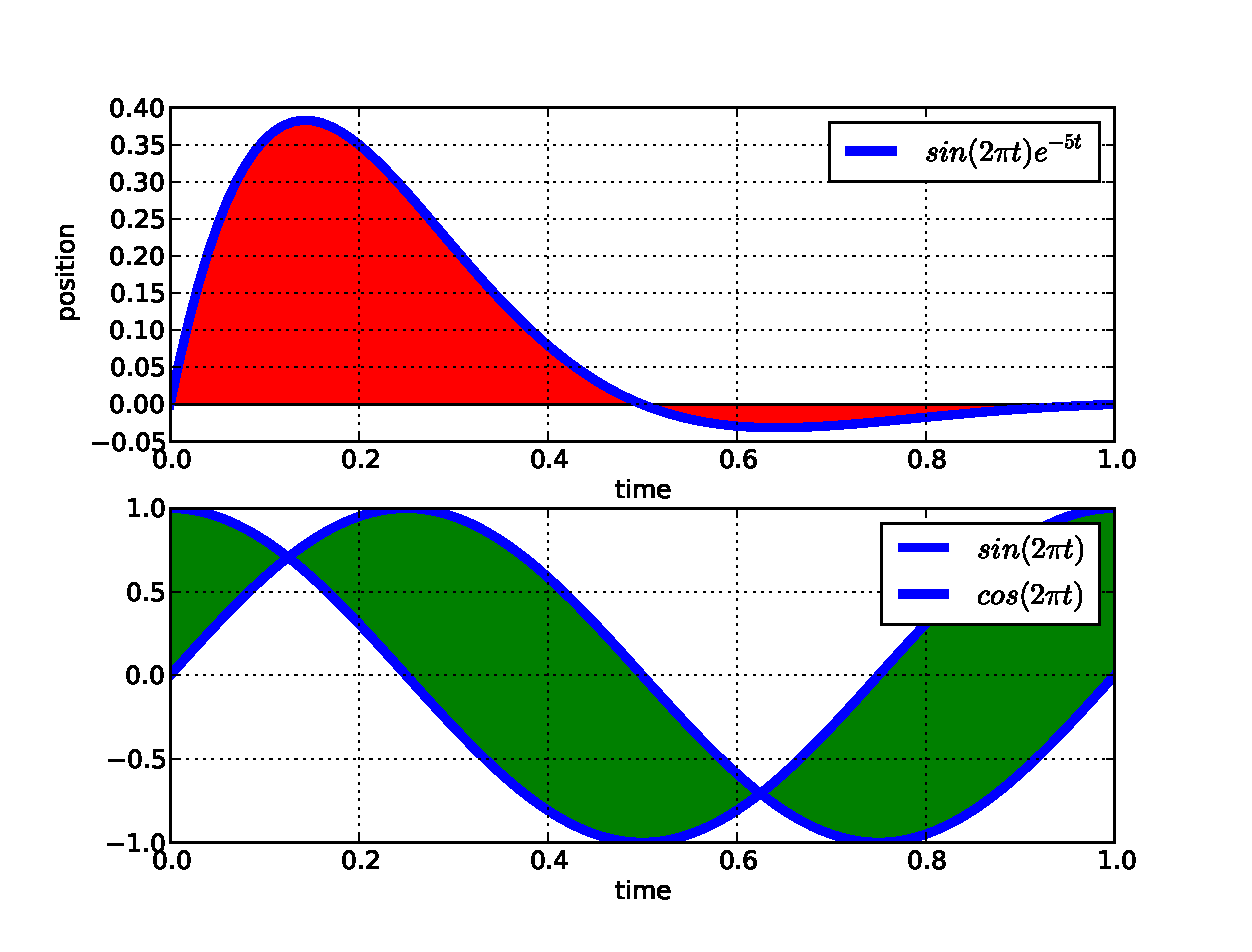
\includegraphics[width=0.8\textwidth]{pics/simple-plot-2}
\end{figure}
\item[] Helpful functions: {\tt pylab.grid}, {\tt pylab.plot}, {\tt pylab.legend}, {\tt pylab.fill}, {\tt pylab.fill\_between }
\end {enumerate}


\section{Polynomial Fitting (polyfit)}
\begin{enumerate}
 \item Generate data by a polynomial function $f(x) = -3x^3 + 2x -8$
 \item Fit a polynomial (\textbf{scipy.polyfit()}) and recover the coefficients of the polynomial. 
 \item Try the same procedure with noisy data.
(use  \textbf{np.random.randn()} to add noise to the data)
\end{enumerate}

\section{Nonlinear Fitting}
\begin{enumerate}
  \item Define the function $f(x) = e^{-ax} + b$
  \item Generate noisy data from that function with parameters $a = 2., b = 1.4$
  \item Make a simple plot of the data
  \item Use \textbf{scipy.optimize.curve\_fit()} to estimate a and b from the 
data and plot the results.
\end{enumerate}

\section{Intergration}
\begin{enumerate}
  \item Define the function $f(x) = e^{-(x+3)^2}$
  \item Vectorize the function by using \textbf{np.vectorize()} such that 
the function also accepts lists of xvalues.
  \item Calculate the integral $\int_{-20}^{20} f(x)\mathrm{d}x$ by hand, using Riemann sums.
  \item Use \textbf{scipy.integrate.quad()} to evaluate the integral.
  \item Try to calculate $\int_{1}^{\infty} \frac1x \mathrm{d}x$ and $\int_1^\infty \frac1{x^2}\mathrm{d}x$
\end{enumerate}

\section{Solving systems of linear equations}
You find three shopping bags with following content:\\[.5em]
\begin{tabular}{lll}
	bag A: 	&10 kg apples, 5 kg pears, 1 kg oranges 	&(35.35 EUR) \\
	bag B:	&1 kg apples, 8 kg pears, 1 kg oranges	&(24.91 EUR) \\
	bag C: 	&9 kg apples, 3 kg pears, 5 kg oranges	&(40.38 EUR) \\
\end{tabular}
\\[.5em]
Determine the price of apples, oranges and pears.
\begin{enumerate}
  \item Formulate a linear system of equations describing the 	shopping bags.
  \item Use \textbf{scipy.linalg.solve()} to solve the system of equations.
  \item Verify the results by using \textbf{numpy.dot()}.
\end{enumerate}

\section{Some linear algebra}
\begin{enumerate}
\item Create a random matrix, where the entries are randomly chosen from a standard normal (Gaussian) distribution.
\item Plot the (complex!) eigenvalues of that matrix, add labels to the axis and a legend.
\item Add a title for your plot and make it red and increase the size.
\item Store your graph as an {\tt .eps}  file:
\begin{figure}[H]
  \centering
  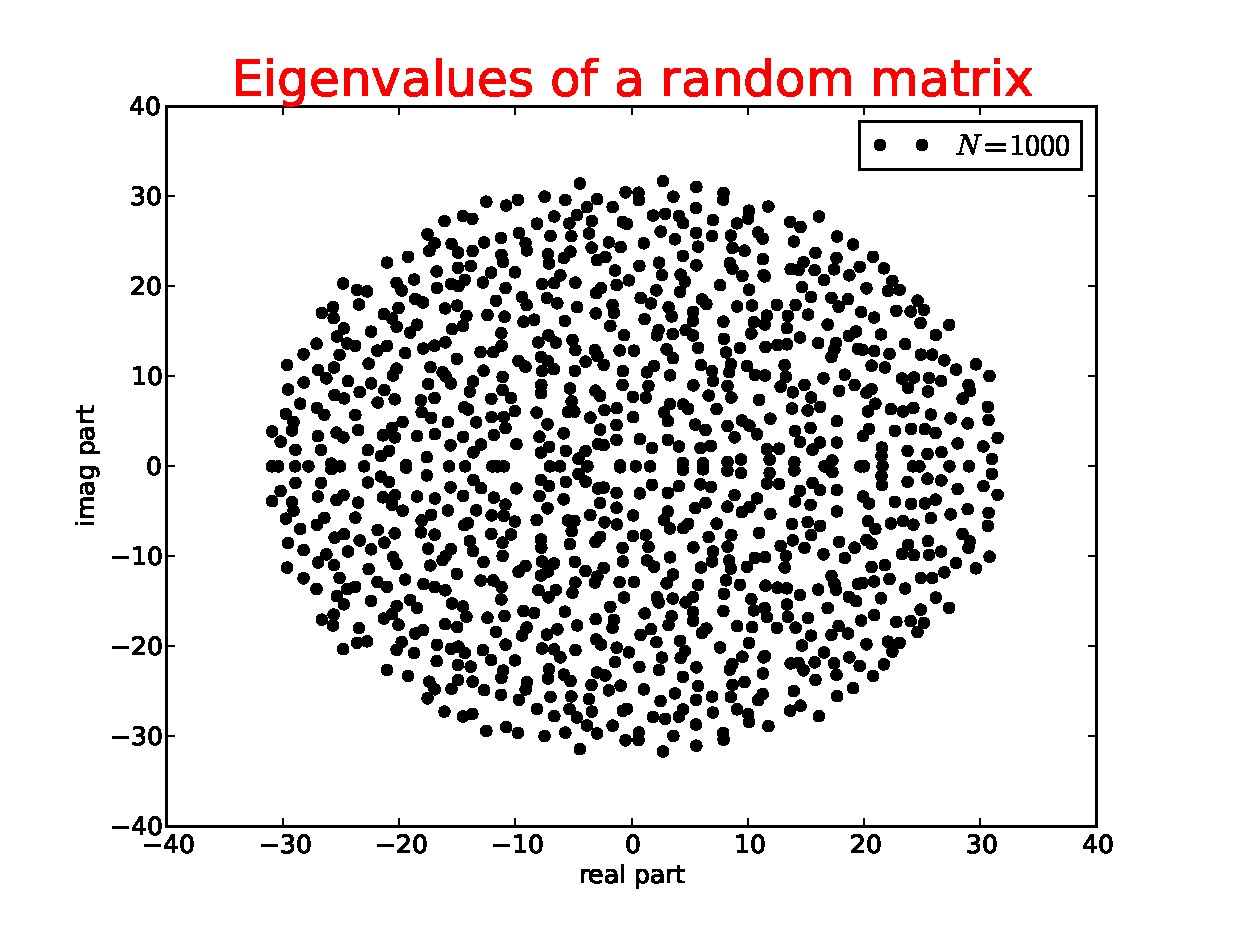
\includegraphics[width=0.8\textwidth]{pics/matrix1}
\end{figure}
\item Define a function that returns {\tt True}  if a point $(x,y)$ is contained in a circle of radius $r$ around the origin.
\item Define a function to find the smallest circle containing all the eigenvalues of your matrix.
\item Plot the eigenvalues for a matrix of size $N=50,100,200,500$ together with the smallest disc containing the eigenvalues.
Therefore first import the {\tt matplotlib} module {\tt matplotlib.patch} and have a look at the classes contained in that module. 
Having identified a suitable class create a patch (a circle) and try to add it to your plot. (Hint: Patches can be added to axes objects)
\begin{figure}[H]
  \centering
  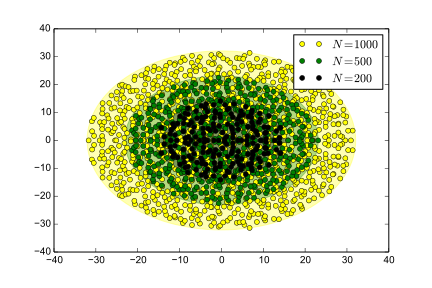
\includegraphics[width=0.8\textwidth]{pics/matrix2}
\end{figure}

\item[] Helpful functions: {\tt scipy.linalg.eigenvals}, {\tt numpy.real}, {\tt numpy.imag}
\end{enumerate}

\section{Calculating a Histogram}

\begin{enumerate}
\item Take the histogram function {\tt histgram( data, numbins )} from the basic-exercises sheet 2. \\
Modify the function, such that its output is now a tuple of numpy arrays. it 
returns an array containing the left border of each bin, an array with the number of data points in each bin 
and the bin width. 
\item Use this function to create a graphical histogram using {\tt pylab.bar()}.
Compare your results with the plot generated by {\tt pylab.histogram()}.
\end{enumerate}



\section{1D Arrays and Plotting}
\begin{enumerate}
\item Plot a 1D Gaussian probability density function with $\mu=10$ and $\sigma=5$ using the formula
  \[
  G(x) = \frac{1}{\sqrt{2\pi}\sigma} \exp\left( \frac{-(x-\mu)^2}{2\sigma^2} \right)
  \]
  Choose a suitable $x$-range.

\item Use a numerical integration method to calculate the integral of
  $G(x)$ on the interval $[\mu-50,\mu+50]$ and verify that it is
  approximately equal to 1
\item Integrate the function with varying window sizes $w_i$, such that the
  integration is on the interval $[\mu-w_i, \mu+w_i]$. Plot the
  integral as a function of the used window-size.
\item[] Helpful functions: {\tt numpy.arange, pylab.plot, scipy.integrate.quad}
\end{enumerate}

\section{2D Arrays and Plotting}
\begin{enumerate}
\item Calculate a bivariate standard normal density
\[
G_2(x,y) = \frac{1}{\sqrt{2\pi}} \exp\left( \frac{-(x^2+y^2)}{2}\right)
\]
on the interval $[-3,3]$ and save it to a matrix {\tt G}.
\item Plot the result in an image with a colorbar-legend.
\item The bivariate gaussian has a hat-like shape. Use index-slicing
  to get $4$ separate, nonoverlapping matrices {\tt Q1,Q2,Q3,Q4}
  (quadrants) of equal dimensions that cover the whole matrix {\tt
    G}. Create a new matrix {\tt G2} in which {\tt Q1} and {\tt Q3}
  changed place and {\tt Q2} $\leftrightarrow$ {\tt Q4}. Plot this
  result as well.
\item Plot the difference of {\tt G} and {\tt G2}.
\item[] Functions to use: {\tt numpy.arange}, {\tt numpy.meshgrid}, 
  {\tt pylab.imshow}, {\tt pylab.colorbar}, {\tt numpy.empty}
\end{enumerate}

\section{Calculate a Power spectrum }
Away to look at a signal is to view its spectral density (i.e., the Fourier transform of the signal). The Fourier transform views the signal as a whole. It swaps the dimension of time with the dimension of frequency. One can think of the Fourier transform as a combination of slow and fast oscillations with different amplitude. A very strong and slow component in the frequency domain implies that there is a high correlation between the large-scale pieces of the signal in time (macro-structures), while a very strong and fast oscillation implies correlation in the micro-structures. Therefore, if our signal $ f(t) $ represents values in every single moment of time, its Fourier transform $F(\omega)$ represents the strength of every oscillation in a holistic way in that chunk of time. These two signals are related to each other by the following formula:
$\displaystyle F(\omega) = \int_{-\infty}^{\infty} f(t){e}^{-j\omega t} dt.$ 

For simplicity, in the following we will consider a signal that is constructed by summing different sine waves and try to get information about the underlying frequencies.
\begin{enumerate}
 \item Construct a signal by adding $20$ sine waves with a frequency randomly choosen from the interval $[1Hz, 300Hz]$.
 \item Plot the signal in the interval $t=0,...,2s$.
 \item Use numpy to calculate the one-dimensional discrete Fourier Transform.
 \item The square of the absolute value of the fourier transform gives you the power carried by each frequency (power spectrum). To calculate the Fourier transform sample frequencies you can also use numpy function - have a look at the documentation of the numpy.fft module. Plot the powerspectrum and also indicate the frequencies that were used for generating the data.
 \item Add a plot of the original time series to the plot of the power spectrum. To generate the subplot you can add an axes object directly to the figure. If you don't know how to do that have a look at the documentation of matplotlib or the examples in the gallery (http://matplotlib.sourceforge.net/gallery.html).

\begin{figure}[H]
  \centering
  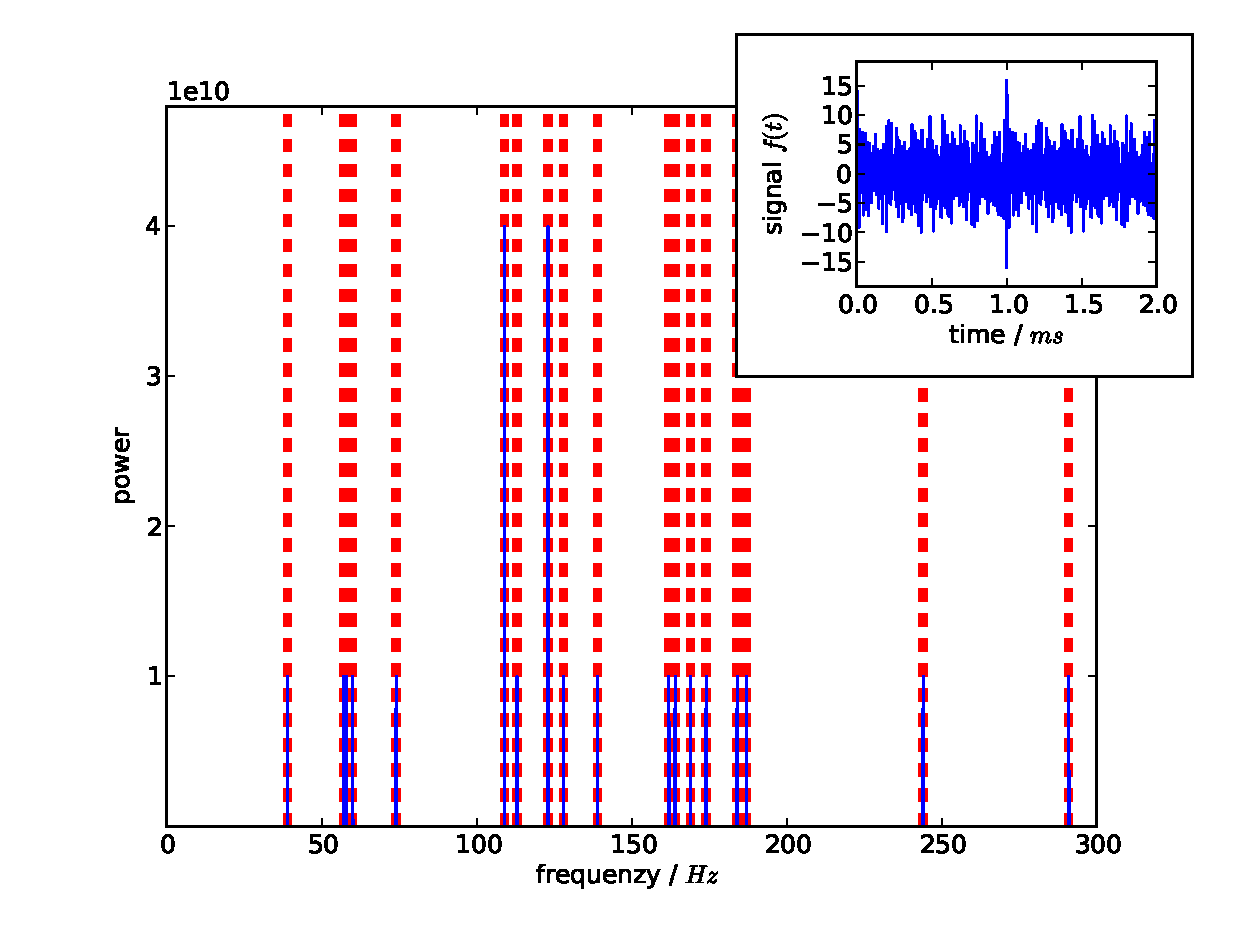
\includegraphics[width=0.8\textwidth]{pics/power}
\end{figure}
 
\end{enumerate}

\section{Vectorization of Monte-Carlo Simulation}
Recall the dice-simulation from the basic-exercise sheet. The goal of
the current exercise is to optimize this program using vectorization.
\begin{enumerate}
\item Create a script that $N$-times draws two uniform random integers
  from 1 to 6 and counts how many times $X$ at least one of the two takes
  the value 6. Do this
  in a single $N\times 2$ matrix.  Write out the estimated probability
  $X/N$ together with the exact result $11/36$.
\item Run this simulation for growing $N$ and plot the estimated probability as a
  function of $N$. Try to use linear and logarithmic axis.
\item Repeat the dice throwing $Z$ times for a fixed value of $N$ and
plot a histogram of the number of throws with at  least one six (e.g. for $N=1000$, $Z=10000$). 
\item The data are integers, so choose a bin width of $1$. Further print out the mean value and the standard deviation.
\item As above repeat the dice throwing for a fixed number $N$ of dice throws $Z$ times and calculate the probability 
to get at least one six with the two dices. From this data you can calculate the empirical average and standard 
deviation for every pair of $N$ and $Z$. Make an error-bar plot for $N=1,\ldots,20$ and $Z=5000$.

\item[] Helpful functions: {\tt numpy.random.randint}, {\tt numpy.sum}, {\tt numpy.vectorize}, {\tt numpy.mean}
{\tt numpy.std}, {\tt pylab.plot}, {\tt pylab.semilogx}, {\tt pylab.hist}
\end{enumerate}

%\section*{One Curve Fitting example}
\section{ODE integration}
Recall the Neuron Class from last week. There you approximated the time derivative of the membrane potential by
\[ \dot{V}\approx\frac{V(t+h)-V(t)}{h} \textup{ .} \]
\begin{enumerate}
 \item Now use the methods from {\tt numpy.integrate} to provide a more accurate integral of the equation determining 
the membrane potential
\[c_{M}\dot{V}=-g_{L}\left(V-V_{L}\right)+i_{ext}\]

 \end{enumerate}
% \newpage
\section{Lotka-Voltera System}
Consider the Lotka-Voltera equation of predator-prey interactions\\[0.5em]
$\frac{\mathrm{d}N_1}{\mathrm{d}t} = N_1(\epsilon_1 - \gamma_1 N_2),$\\
$\frac{\mathrm{d}N_2}{\mathrm{d}t} = -N_2(\epsilon_2 - \gamma_2 N_2)$\\[0.5em]
This is a system of ordinary differential equations, where $N_1(t)$ is the number of preys and $N_2(t)$ the number of predators.
$\epsilon_1,\:\epsilon_2,\:\gamma_1,\:\gamma_2$ are parameters representing the growth and interaction between preys and predators.
\begin{enumerate}
  \item Find the fixed points of the system for the following parameters\\
$\epsilon_1 = 1.0,\:\epsilon_2 = 1.5,\:\gamma_1 = 0.1,\:\gamma_2 = 0.075$
    \begin{itemize}
      \item Define a function that returns the growing rates $\frac{\mathrm{d}N_1}{\mathrm{d}t}$ and $\frac{\mathrm{d}N_1}{\mathrm{d}t}$ in an array. In the second part of the exercise, we will use \textbf{scipy.integrate.odeint()} to obtain the solution of the ODE system. Therefore,  choose the parameters of your function accordingly, $f = f(N, t, ...)$.
      \item Use \textbf{scipy.optimize.fsolve()} to find the fixed points of the system.
    \end{itemize}

  \item Solve the system of equations for the following initial conditions:\\ $N_1(0) = 10,\:N_2(0) = 5$
    \begin{itemize}
      \item Define a vector containing the time steps of the integration and one for the initial conditions.
      \item Solve the system, using \textbf{scipy.integrate.odeint()}.
      \item Plot the results for two different time step sizes.
    \end{itemize}
\begin{figure}[H]
  \centering
  \includegraphics[width=0.8\textwidth]{pics/LottkaVoltera.png}
\end{figure}

\end{enumerate}
% the last two points are more defined in the presentation...

\end{document}
